\documentclass[aspectratio=169]{beamer}
\usetheme{Boadilla}
%\usetheme{Warsaw}
%\setbeamercovered{transparent}
\beamertemplatetransparentcoveredhigh
\usepackage[portuges]{babel}
\usepackage[utf8]{inputenc}
\usepackage{lmodern}
\usepackage[T1]{fontenc}
\usepackage[portuguese, linesnumbered, vlined, titlenumbered, ruled]{algorithm2e}
\SetKwRepeat{Registro}{registro \{}{\}}%
\usepackage{hyperref} 

\usepackage{xcolor}

\definecolor{codegreen}{rgb}{0,0.6,0}
\definecolor{codegray}{rgb}{0.5,0.5,0.5}
\definecolor{codepurple}{rgb}{0.58,0,0.82}
\definecolor{backcolour}{rgb}{0.95,0.95,0.92}

\usepackage{listings}
\lstdefinestyle{CStyle}{
    language=C++,
    backgroundcolor=\color{backcolour},   
    commentstyle=\color{codegreen},
    keywordstyle=\color{magenta},
    numberstyle=\tiny\color{codegray},
    stringstyle=\color{codepurple},
    basicstyle=\ttfamily\footnotesize,
    breakatwhitespace=false,         
    breaklines=true,                 
    keepspaces=true,                 
    numbers=left,       
    numbersep=5pt,                  
    showspaces=false,                
    showstringspaces=false,
    showtabs=false,                  
    tabsize=2,
}

\newcommand{\eng}[1]{\textsl{#1}}
\newcommand{\cod}[1]{\texttt{#1}}

\title[Aula Prática - Árvores Binárias de Busca]{Algoritmos e Estrutura de Dados}
\subtitle{Árvores Binárias de Busca}
\author[Frederico Santos de Oliveira]{prof. Frederico Santos de Oliveira}
\institute[UFMT]{Universidade Federal de Mato Grosso\\ Faculdade de Engenharia}
\date{}

\begin{document}

\begin{frame}[plain]
  \titlepage
\end{frame}

%\section*{Roteiro}

\begin{frame}
  \frametitle{Agenda}
  \tableofcontents
\end{frame}

%%%%%%%%%%%%%%%%%%%%%%%%%%%%%%%%%%%%%%%%%%%%%%%%%%%%%%%%%%%%%%%%%%%%%%%%%%%%%%%%%%%%%%%%%%%%%%%%%%%%%%%%%

\begin{frame}
\frametitle{Exercício}
Vamos implementar a estrutura de dados Árvore Binária de Busca (ABB).
\end{frame}

%%%%%%%%%%%%%%%%%%%%%%%%%%%%%%%%%%%%%%%%%%%%%%%%%%%%%%%%%%%%%%%%%%%%%%%%%%%%%%%%%%%%%%%%%%%%%%%%%%%%%%%%%
\section{Estrutura Nodo}
%%%%%%%%%%%%%%%%%%%%%%%%%%%%%%%%%%%%%%%%%%%%%%%%%%%%%%%%%%%%%%%%%%%%%%%%%%%%%%%%%%%%%%%%%%%%%%%%%%%%%%%%%

\begin{frame}{Árvore Binária}{Implementação}
Uma ABB é formada pela estrutura {\bf nodo}, que contém três campos:
\begin{itemize}
 \item Um ponteiro {\bf esq}, que indica o filho da esquerda daquele nodo.
 \item Um ponteiro {\bf dir}, que indica o filho da direita daquele nodo.
 \item Um campo {\bf item} do tipo {\bf int}, que é o tipo de dado a ser armazenado no nodo da árvore.
\end{itemize}
\begin{figure}[!h]
  \centering
  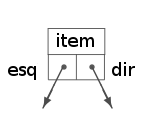
\includegraphics[width=70pt]{imagens/nodo.png}
  \label{fig_nodo}
\end{figure}
\end{frame}

%%%%%%%%%%%%%%%%%%%%%%%%%%%%%%%%%%%%%%%%%%%%%%%%%%%%%%%%%%%%%%%%%%%%%%%%%%%%%%%%%%%%%%%%%%%%%%%%%%%%%%%%%

\begin{frame}[fragile]{Árvore Binária}{Estrutura Nodo}
Segue o pseudo-código referente à estrutura nodo:
\begin{algorithm}[H]
\caption{Nodo} 
\label{Nodo}
\Inicio{
 \Registro{Nodo}{
    Inteiro: item; \\
    Ponteiro Nodo: esq; \\
    Ponteiro Nodo: dir; 
  }
}
\end{algorithm} 
\end{frame}

%%%%%%%%%%%%%%%%%%%%%%%%%%%%%%%%%%%%%%%%%%%%%%%%%%%%%%%%%%%%%%%%%%%%%%%%%%%%%%%%%%%%%%%%%%%%%%%%%%%%%

\begin{frame}[fragile]{Árvore Binária}{Estrutura Nodo}
Na linguagem C, a implementação fica conforme o código a seguir:
\begin{lstlisting}[style=CStyle]
typedef struct nodo_t
{
    int item;
    struct nodo_t *esq;
    struct nodo_t *dir;
} nodo;
\end{lstlisting}  
\end{frame}

%%%%%%%%%%%%%%%%%%%%%%%%%%%%%%%%%%%%%%%%%%%%%%%%%%%%%%%%%%%%%%%%%%%%%%%%%%%%%%%%%%%%%%%%%%%%%%%%%%%%%
\section{Estrutura Árvore Binária}
%%%%%%%%%%%%%%%%%%%%%%%%%%%%%%%%%%%%%%%%%%%%%%%%%%%%%%%%%%%%%%%%%%%%%%%%%%%%%%%%%%%%%%%%%%%%%%%%%%%%%

\begin{frame}{Árvore Binária}{Estrutura Árvore}
A estrutura {\bf árvore} trata-se de um ponteiro do tipo {\bf nodo}:
\begin{itemize}
 \item O ponteiro {\bf raiz} aponta para o nodo raiz da árvore.
 \item Se a árvore está vazia, o ponteiro {\bf raiz} aponta para NULL.
\end{itemize}
\begin{figure}[!h]
  \centering
  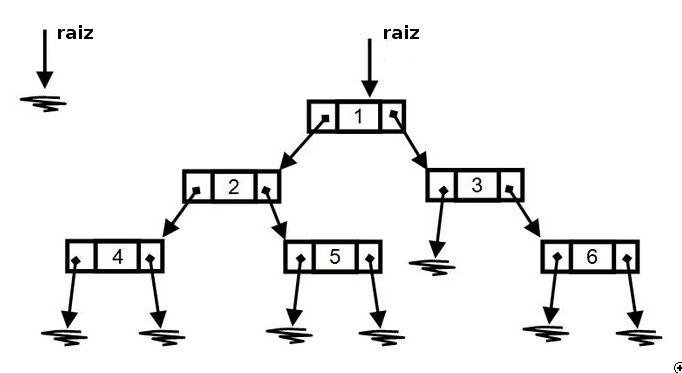
\includegraphics[width=300pt]{imagens/estrutura_arvore.png}
  \label{fig_estrutura_arvore}
\end{figure}
\end{frame}

%%%%%%%%%%%%%%%%%%%%%%%%%%%%%%%%%%%%%%%%%%%%%%%%%%%%%%%%%%%%%%%%%%%%%%%%%%%%%%%%%%%%%%%%%%%%%%%%%%%%%

\begin{frame}[fragile]{Árvore Binária}{Estrutura Árvore}
\begin{algorithm}[H]
\caption{Arvore} 
\label{Arvore}
\Inicio{
 Tipo Nodo* Arvore;
}
\end{algorithm} 
Na linguagem C, a implementação fica conforme o código a seguir:
\begin{lstlisting}[style=CStyle]
typedef nodo* Arvore;
\end{lstlisting}  

\end{frame}



%%%%%%%%%%%%%%%%%%%%%%%%%%%%%%%%%%%%%%%%%%%%%%%%%%%%%%%%%%%%%%%%%%%%%%%%%%%%%%%%%%%%%%%%%%%%%%%%%%%%%
\begin{frame}{Árvore Binária de Busca}{Inserção}
Agora, vamos implementar dois algoritmos básicos:
\begin{itemize}
 \item {\bf CriaÁrvore}: cria uma árvore vazia.
 \item {\bf ArvoreVazia}: verifica se uma árvore está vazia.
\end{itemize}
\end{frame}
%%%%%%%%%%%%%%%%%%%%%%%%%%%%%%%%%%%%%%%%%%%%%%%%%%%%%%%%%%%%%%%%%%%%%%%%%%%%%%%%%%%%%%%%%%%%%%%%%%%%%
\section{Criar Árvore | Árvore Vazia}
%%%%%%%%%%%%%%%%%%%%%%%%%%%%%%%%%%%%%%%%%%%%%%%%%%%%%%%%%%%%%%%%%%%%%%%%%%%%%%%%%%%%%%%%%%%%%%%%%%%%%

\begin{frame}{Árvore Binária}{Implementação}
% \scalebox{0.5}{
\begin{algorithm}[H]
\caption{CriaÁrvore} 
\label{CriaArvore}
\Saida{Ponteiro $r$ para raiz.}
\Inicio{
    r $\leftarrow$ NULL 
}
\end{algorithm}
% }  
\begin{algorithm}[H]
\caption{ÁrvoreVazia} 
\label{ArvoreVazia}
\Entrada{Ponteiro $r$ para raiz.}
\Saida{V ou F}
\Inicio{
  \Retorna (r = NULL)
  
}
\end{algorithm}
% }  
\end{frame}

%%%%%%%%%%%%%%%%%%%%%%%%%%%%%%%%%%%%%%%%%%%%%%%%%%%%%%%%%%%%%%%%%%%%%%%%%%%%%%%%%%%%%%%%%%%%%%%%%%%%%

\begin{frame}[fragile]{Árvore Binária}{Estrutura Árvore}
Na linguagem C, a implementação dessas funções fica conforme o código a seguir:
\begin{lstlisting}[style=CStyle]
Arvore* cria_arvore() {
    Arvore* raiz = (Arvore*) malloc(sizeof(Arvore));
    if(raiz != NULL)
        *raiz = NULL;
    return raiz;   
}

int arvore_vazia(nodo *r) {
    return r == NULL;
}
\end{lstlisting}  
\end{frame}

%%%%%%%%%%%%%%%%%%%%%%%%%%%%%%%%%%%%%%%%%%%%%%%%%%%%%%%%%%%%%%%%%%%%%%%%%%%%%%%%%%%%%%%%%%%%%%%%%%%%%
\section{Inserção}
%%%%%%%%%%%%%%%%%%%%%%%%%%%%%%%%%%%%%%%%%%%%%%%%%%%%%%%%%%%%%%%%%%%%%%%%%%%%%%%%%%%%%%%%%%%%%%%%%%%%%

\begin{frame}{Inserção}{Introdução}
Agora, vamos implementar um algoritmo para {\bf inserir} dados na nossa árvore. Podemos implementar duas versões:
\begin{itemize}
 \item {\bf Recursiva}: utiliza chamadas recursivas.
 \item {\bf Iterativa}: utiliza laços de repetição.
\end{itemize}
\end{frame}

%%%%%%%%%%%%%%%%%%%%%%%%%%%%%%%%%%%%%%%%%%%%%%%%%%%%%%%%%%%%%%%%%%%%%%%%%%%%%%%%%%%%%%%%%%%%%%%%%%%%%

\begin{frame}{Inserção}{Pseudo-Código Versão Recursiva}
% \scalebox{0.8}{
\begin{algorithm}[H]
\caption{InserirÁrvore} 
\label{InserirArvore}
\Entrada{Ponteiro $r$ para raiz, item $x$ a ser inserido na árvore.}
\Inicio{
  \Se{(r=NULL)} {
    novo $\leftarrow$ ALOCA\_NODO() \\
    novo.item $\leftarrow$ x \\
    novo.esq $\leftarrow$ NULL \\
    novo.dir $\leftarrow$ NULL \\               
    r $\leftarrow$ novo \\ 
  }
  \Se {(x $<$ r.item)} {
      InserirÁrvore(r.esq, x) \\
  } 
  \Senao {
      InserirÁrvore(r.dir, x) \\
  }
}
\end{algorithm}
% }  
\end{frame}

%%%%%%%%%%%%%%%%%%%%%%%%%%%%%%%%%%%%%%%%%%%%%%%%%%%%%%%%%%%%%%%%%%%%%%%%%%%%%%%%%%%%%%%%%%%%%%%%%%%%%

\begin{frame}[fragile]{Inserção}{Código-Fonte Versão Recursiva}
Na linguagem C, a implementação dessa função fica conforme o código a seguir:
\begin{lstlisting}[style=CStyle,basicstyle=\tiny]
int inserir_arvore_recursivo(Arvore* raiz, int valor){
    if(raiz == NULL)
        return 0;
    nodo* novo;
    novo = (nodo*) malloc(sizeof(nodo));
    if(novo == NULL)
        return 0;
    novo->item = valor;
    novo->dir = NULL;
    novo->esq = NULL;

    if(*raiz == NULL)
        *raiz = novo;
    else{        
        if(valor < (*raiz)->item){
           return inserir_arvore_recursivo(&(*raiz)->esq, valor);
        }
        else
           return inserir_arvore_recursivo(&(*raiz)->dir, valor);
    }
    return 1;
}
\end{lstlisting}  
\end{frame}

%%%%%%%%%%%%%%%%%%%%%%%%%%%%%%%%%%%%%%%%%%%%%%%%%%%%%%%%%%%%%%%%%%%%%%%%%%%%%%%%%%%%%%%%%%%%%%%%%%%%%

\begin{frame}{Inserção}{Pseudo-Código Versão Iterativa}
\scalebox{0.5}{
\begin{algorithm}[H]
\caption{InserirÁrvore} 
\label{InserirArvoreIte}
\Entrada{Ponteiro $r$ para raiz, item $x$ a ser inserido na árvore.}
\Inicio{
  novo $\leftarrow$ ALOCA\_NODO() \\
  novo.item $\leftarrow$ x \\
  novo.esq $\leftarrow$ NULL \\
  novo.dir $\leftarrow$ NULL \\             
  \Se{(r=NULL)} {
    r $\leftarrow$ novo \\ 
  }
  \Senao {
    atual $\leftarrow$ r \\
    anterior $\leftarrow$ NULL \\
    \Enqto{(atual $\neq$ NULL)} {
      anterior $\leftarrow$ atual \\
      \Se {(novo.item $<$ atual.item)} {
	atual $\leftarrow$ atual.esq \\
      } 
      \Senao {
	atual $\leftarrow$ atual.dir \\
      }
    }
    \Se {(novo.item $<$ anterior.item)} {
      anterior.esq $\leftarrow$ novo \\
    }
    \Senao {
      anterior.dir $\leftarrow$ novo \\
    }
  }
}
\end{algorithm}
}  
\end{frame}

%%%%%%%%%%%%%%%%%%%%%%%%%%%%%%%%%%%%%%%%%%%%%%%%%%%%%%%%%%%%%%%%%%%%%%%%%%%%%%%%%%%%%%%%%%%%%%%%%%%%%

\begin{frame}[fragile]{Inserção}{Código-Fonte Versão Iterativa - Parte 1}
Na linguagem C, a implementação dessa função fica conforme o código a seguir:
\begin{lstlisting}[style=CStyle,basicstyle=\tiny]
int inserir_arvore_iterativo(Arvore* raiz, int valor){
    if(raiz == NULL)
        return 0;
    nodo* novo;
    novo = (nodo*) malloc(sizeof(nodo));
    if(novo == NULL)
        return 0;
    novo->item = valor;
    novo->dir = NULL;
    novo->esq = NULL;

    if(*raiz == NULL)
        *raiz = novo;
        /** continua no proximo slide **/  
\end{lstlisting}  
\end{frame}

%%%%%%%%%%%%%%%%%%%%%%%%%%%%%%%%%%%%%%%%%%%%%%%%%%%%%%%%%%%%%%%%%%%%%%%%%%%%%%%%%%%%%%%%%%%%%%%%%%%%%

\begin{frame}[fragile]{Inserção}{Código-Fonte Versão Iterativa - Parte 2}
\begin{lstlisting}[style=CStyle,basicstyle=\tiny,firstnumber=12]
    if(*raiz == NULL)
        *raiz = novo;        
    /** slide anterior **/
    else {
        nodo* atual = *raiz;
        nodo* ant = NULL;
        while (atual != NULL) {
            ant = atual;
            if(valor == atual->item) {
                free(novo);
                return 0;
            }

            if(valor > atual->item)
                atual = atual->dir;
            else
                atual = atual->esq;
        }
        if(valor > ant->item)
            ant->dir = novo;
        else
            ant->esq = novo;
    }
    return 1;
}  
\end{lstlisting}  
\end{frame}

%%%%%%%%%%%%%%%%%%%%%%%%%%%%%%%%%%%%%%%%%%%%%%%%%%%%%%%%%%%%%%%%%%%%%%%%%%%%%%%%%%%%%%%%%%%%%%%%%%%%%
\section{Quantidade de Nodos}
%%%%%%%%%%%%%%%%%%%%%%%%%%%%%%%%%%%%%%%%%%%%%%%%%%%%%%%%%%%%%%%%%%%%%%%%%%%%%%%%%%%%%%%%%%%%%%%%%%%%%

\begin{frame}[fragile]{Quantidade de Nodos}{Introdução}
Vamos implementar um algoritmo que calcula a {\bf quantidade de nodos} na nossa árvore.
\end{frame}

%%%%%%%%%%%%%%%%%%%%%%%%%%%%%%%%%%%%%%%%%%%%%%%%%%%%%%%%%%%%%%%%%%%%%%%%%%%%%%%%%%%%%%%%%%%%%%%%%%%%%

\begin{frame}[fragile]{Quantidade de Nodos}{Introdução}
A quantidade de nodos em uma árvore com raiz em $r$ é calculada da seguinte forma:
 \begin{itemize}
 \item Verifica se $r$ é vazio. 
 \begin{itemize}
 \item Caso sim, a quantidade de nodos é zero.
 \item Caso contrário, o total de nodos da árvore com raiz em $r$ será a soma da quantidade de nodos em suas subárvores mais um (referente ao nodo raiz $r$).
 \end{itemize} 
 \item A seguir, o pseudocódigo.
 \end{itemize} 
\end{frame}

%%%%%%%%%%%%%%%%%%%%%%%%%%%%%%%%%%%%%%%%%%%%%%%%%%%%%%%%%%%%%%%%%%%%%%%%%%%%%%%%%%%%%%%%%%%%%%%%%%%%%

\begin{frame}[fragile]{Quantidade de Nodos}{Pseudo-Código}
% \scalebox{0.5}{
\begin{algorithm}[H]
\caption{QuantidadeNodos} 
\label{QuantidadeNodos}
\Entrada{Ponteiro $r$ para raiz.}
\Saida{Quantidade de nodos em $r$.}
\Inicio{
  \Se {(r = NULL)} {
    \Retorna 0
  }
  \Senao {
    total\_esq $\leftarrow$ QuantidadeNodos($r$.esq) \\
    total\_dir $\leftarrow$ QuantidadeNodos($r$.dir) \\
    \Retorna total\_esq + total\_dir + 1
  }
}
\end{algorithm}
% }  
\end{frame}

%%%%%%%%%%%%%%%%%%%%%%%%%%%%%%%%%%%%%%%%%%%%%%%%%%%%%%%%%%%%%%%%%%%%%%%%%%%%%%%%%%%%%%%%%%%%%%%%%%%%%

\begin{frame}[fragile]{Quantidade de Nodos}{Código-Fonte}
\begin{lstlisting}[style=CStyle,basicstyle=\small]
int quantidade_nodos(nodo *r) {
    if (r == NULL)
        return 0;
    else {
        int t_esq = quantidade_nodos(r->esq);
        int t_dir = quantidade_nodos(r->dir);
        return t_esq + t_dir + 1;
    }
} 
\end{lstlisting}  
\end{frame}

%%%%%%%%%%%%%%%%%%%%%%%%%%%%%%%%%%%%%%%%%%%%%%%%%%%%%%%%%%%%%%%%%%%%%%%%%%%%%%%%%%%%%%%%%%%%%%%%%%%%%
\section{Altura}
%%%%%%%%%%%%%%%%%%%%%%%%%%%%%%%%%%%%%%%%%%%%%%%%%%%%%%%%%%%%%%%%%%%%%%%%%%%%%%%%%%%%%%%%%%%%%%%%%%%%%

\begin{frame}{Altura}{Introdução}
Vamos implementar um algoritmo que calcula a {\bf altura} da nossa árvore.
\end{frame}

%%%%%%%%%%%%%%%%%%%%%%%%%%%%%%%%%%%%%%%%%%%%%%%%%%%%%%%%%%%%%%%%%%%%%%%%%%%%%%%%%%%%%%%%%%%%%%%%%%%%%

\begin{frame}{Altura}{Introdução}
A altura é calculada da seguinte forma:
 \begin{itemize}
 \item Verifica se o nodo é um nodo folha. 
 \begin{itemize}
 \item Caso sim, sua altura é zero.
 \item Caso contrário, obtém-se a maior altura entre suas subárvores, e incrementa em um.
 \end{itemize} 
 \item A seguir, o pseudocódigo.
 \end{itemize} 
\end{frame}

%%%%%%%%%%%%%%%%%%%%%%%%%%%%%%%%%%%%%%%%%%%%%%%%%%%%%%%%%%%%%%%%%%%%%%%%%%%%%%%%%%%%%%%%%%%%%%%%%%%%%

\begin{frame}{Altura}{Pseudo-Código}
% \scalebox{0.5}{
\begin{algorithm}[H]
\caption{AlturaÁrvore} 
\label{AlturaArvore}
\Entrada{Ponteiro $r$ para raiz.}
\Saida{Altura da árvore com raiz em $r$.}
\Inicio{
  \Se {(r = NULL)} {
    \Retorna -1
  }
  \Senao {
    alt\_esq $\leftarrow$ AlturaÁrvore($r$.esq) \\
    alt\_dir $\leftarrow$ AlturaÁrvore($r$.dir) \\
    \Se {(alt\_esq $>$ alt\_dir)} {
      \Retorna alt\_esq + 1
    }
    \Senao {
      \Retorna alt\_dir + 1
    }
  }
}
\end{algorithm}
% }  
\end{frame}


%%%%%%%%%%%%%%%%%%%%%%%%%%%%%%%%%%%%%%%%%%%%%%%%%%%%%%%%%%%%%%%%%%%%%%%%%%%%%%%%%%%%%%%%%%%%%%%%%%%%%

\begin{frame}[fragile]{Altura}{Código-Fonte}
\begin{lstlisting}[style=CStyle,basicstyle=\small]
int altura_arvore(nodo *r) {
    if (r==NULL)
        return -1;
    else {
        int alt_esq = altura_arvore(r->esq);
        int alt_dir = altura_arvore(r->dir);
        if (alt_esq > alt_dir) 
            return alt_esq + 1;
        else
            return alt_dir + 1;
    }
}
\end{lstlisting}  
\end{frame}

%%%%%%%%%%%%%%%%%%%%%%%%%%%%%%%%%%%%%%%%%%%%%%%%%%%%%%%%%%%%%%%%%%%%%%%%%%%%%%%%%%%%%%%%%%%%%%%%%%%%%
\section{Percurso}
%%%%%%%%%%%%%%%%%%%%%%%%%%%%%%%%%%%%%%%%%%%%%%%%%%%%%%%%%%%%%%%%%%%%%%%%%%%%%%%%%%%%%%%%%%%%%%%%%%%%%

\begin{frame}{Percurso}{Introdução}
Vamos implementar os algoritmos que percorrem uma árvore. São eles:
 \begin{itemize}
 \item Percurso {\bf pré-ordem}: visita a raiz, o filho da esquerda e o filho da direita.
 \item Percurso {\bf em-ordem}: visita o filho da esquerda, a raiz e o filho da direita.
 \item Percurso {\bf pós-ordem}: visita o filho da esquerda, o filho da direita e a raiz.
 \end{itemize} 
\end{frame}

%%%%%%%%%%%%%%%%%%%%%%%%%%%%%%%%%%%%%%%%%%%%%%%%%%%%%%%%%%%%%%%%%%%%%%%%%%%%%%%%%%%%%%%%%%%%%%%%%%%%%

\begin{frame}{Percurso PreOrdem}{Pseudo-Código}
% \scalebox{0.5}{
\begin{algorithm}[H]
\caption{PercursoPréOrdem} 
\label{PercursoPreOrdem}
\Entrada{Ponteiro $r$ para raiz.}
\Inicio{
  \Se {(r $\neq$ NULL)} {
    Imprima (r.item) \\
    PercursoPréOrdem(r.esq)\\
    PercursoPréOrdem(r.dir)\\
  }
}
\end{algorithm}
% }  
\end{frame}

%%%%%%%%%%%%%%%%%%%%%%%%%%%%%%%%%%%%%%%%%%%%%%%%%%%%%%%%%%%%%%%%%%%%%%%%%%%%%%%%%%%%%%%%%%%%%%%%%%%%%

\begin{frame}[fragile]{Percurso PreOrdem}{Código-Fonte}
\begin{lstlisting}[style=CStyle,basicstyle=\small]
void pre_ordem(Arvore *raiz){
    if(raiz == NULL)
        return;
    if(*raiz != NULL){
        printf("%d ",(*raiz)->item);
        pre_ordem(&((*raiz)->esq));
        pre_ordem(&((*raiz)->dir));
    }
}
\end{lstlisting}  
\end{frame}

%%%%%%%%%%%%%%%%%%%%%%%%%%%%%%%%%%%%%%%%%%%%%%%%%%%%%%%%%%%%%%%%%%%%%%%%%%%%%%%%%%%%%%%%%%%%%%%%%%%%%

\begin{frame}{Percurso EmOrdem}{Pseudo-Código}
% \scalebox{0.5}{
\begin{algorithm}[H]
\caption{PercursoEmOrdem} 
\label{PercursoEmOrdem}
\Entrada{Ponteiro $r$ para raiz.}
\Inicio{
  \Se {(r $\neq$ NULL)} {
    PercursoEmOrdem(r.esq)\\
    Imprima (r.item) \\    
    PercursoEmOrdem(r.dir)\\
  }
}
\end{algorithm}
% }  
\end{frame}

%%%%%%%%%%%%%%%%%%%%%%%%%%%%%%%%%%%%%%%%%%%%%%%%%%%%%%%%%%%%%%%%%%%%%%%%%%%%%%%%%%%%%%%%%%%%%%%%%%%%%

\begin{frame}[fragile]{Percurso EmOrdem}{Código-Fonte}
\begin{lstlisting}[style=CStyle,basicstyle=\small]
void em_ordem(Arvore *raiz){
    if(raiz == NULL)
        return;
    if(*raiz != NULL){
        em_ordem(&((*raiz)->esq));
        printf("%d ",(*raiz)->item);
        em_ordem(&((*raiz)->dir));
    }
}
\end{lstlisting}  
\end{frame}

%%%%%%%%%%%%%%%%%%%%%%%%%%%%%%%%%%%%%%%%%%%%%%%%%%%%%%%%%%%%%%%%%%%%%%%%%%%%%%%%%%%%%%%%%%%%%%%%%%%%%

\begin{frame}{Percurso PósOrdem}{Pseudo-Código}
% \scalebox{0.5}{
\begin{algorithm}[H]
\caption{PercursoPósOrdem} 
\label{PercursoPosOrdem}
\Entrada{Ponteiro $r$ para raiz.}
\Inicio{
  \Se {(r $\neq$ NULL)} {
    PercursoPósOrdem(r.esq)\\ 
    PercursoPósOrdem(r.dir)\\
    Imprima (r.item) \\       
  }
}
\end{algorithm}
% }  
\end{frame}

%%%%%%%%%%%%%%%%%%%%%%%%%%%%%%%%%%%%%%%%%%%%%%%%%%%%%%%%%%%%%%%%%%%%%%%%%%%%%%%%%%%%%%%%%%%%%%%%%%%%%

\begin{frame}[fragile]{Percurso EmOrdem}{Código-Fonte}
\begin{lstlisting}[style=CStyle,basicstyle=\small]
void pos_ordem(Arvore *raiz){
    if(raiz == NULL)
        return;
    if(*raiz != NULL){
        pos_ordem(&((*raiz)->esq));
        pos_ordem(&((*raiz)->dir));
        printf("%d ",(*raiz)->item);
    }
}
\end{lstlisting}  
\end{frame}

%%%%%%%%%%%%%%%%%%%%%%%%%%%%%%%%%%%%%%%%%%%%%%%%%%%%%%%%%%%%%%%%%%%%%%%%%%%%%%%%%%%%%%%%%%%%%%%%%%%%%
\section{Busca}
%%%%%%%%%%%%%%%%%%%%%%%%%%%%%%%%%%%%%%%%%%%%%%%%%%%%%%%%%%%%%%%%%%%%%%%%%%%%%%%%%%%%%%%%%%%%%%%%%%%%%

\begin{frame}{Busca}{Introdução}
Vamos implementar duas versões do algoritmo de {\bf busca}:
\begin{enumerate}
 \item Uma versão {\bf recursiva}
 \item Uma versão {\bf iterativa}
\end{enumerate}
\end{frame}

%%%%%%%%%%%%%%%%%%%%%%%%%%%%%%%%%%%%%%%%%%%%%%%%%%%%%%%%%%%%%%%%%%%%%%%%%%%%%%%%%%%%%%%%%%%%%%%%%%%%%

\begin{frame}{Busca}{Pseudo-Códico Versão Recursiva}
% \scalebox{0.8}{
\begin{algorithm}[H]
\caption{Busca Recursiva} 
\label{Buscar}
\Entrada{Ponteiro para a raiz $r$ e o item $x$ a ser procurado.}
\Saida{Retorna o nodo que contém o item $x$ ou NULL caso não encontrado.}
\Inicio{
    \Se {(r = NULL) ou (x = r.item)} {
      \Retorna r
    }
    \Se{(x $>$ r.item)} {
	  \Retorna Buscar(r.dir)
    } 
    \Se{(x $<$ r.item)} {
	  \Retorna Buscar(r.esq)
    }
}
\end{algorithm}
% }  
\end{frame}

%%%%%%%%%%%%%%%%%%%%%%%%%%%%%%%%%%%%%%%%%%%%%%%%%%%%%%%%%%%%%%%%%%%%%%%%%%%%%%%%%%%%%%%%%%%%%%%%%%%%%

\begin{frame}[fragile]{Busca}{Código-Fonte}
\begin{lstlisting}[style=CStyle,basicstyle=\small]
nodo* buscar_arvore_recursiva(Arvore *raiz, int valor){
    if(raiz == NULL)
        return NULL;
    if (*raiz == NULL || valor == (*raiz)->item)
    	return (*raiz);
    else
        if (valor > (*raiz)->item) 
            return buscar_arvore_recursiva(&((*raiz)->dir), valor);
        else 
            return buscar_arvore_recursiva(&((*raiz)->esq), valor);
    return NULL;
}
\end{lstlisting}  
\end{frame}

%%%%%%%%%%%%%%%%%%%%%%%%%%%%%%%%%%%%%%%%%%%%%%%%%%%%%%%%%%%%%%%%%%%%%%%%%%%%%%%%%%%%%%%%%%%%%%%%%%%%%

\begin{frame}{Busca}{Pseudo-Còdigo Versão Iterativa}
\scalebox{0.8}{
\begin{algorithm}[H]
\caption{Busca Iterativa} 
\label{Buscar_iterativo}
\Entrada{Ponteiro para a raiz $r$ e o item $x$ a ser procurado.}
\Saida{Retorna o nodo que contém o item $x$ ou NULL caso não encontrado.}
\Inicio{
    \Se {(r = NULL)} {
      \Retorna NULL
    }
    \Senao {
      atual $\leftarrow$ r \\
      \Enqto {(atual $\neq$ NULL)} {
	\Se{(x = atual.item)} {
	  \Retorna atual
	}
	\Se{(x $>$ atual.item)} {
	  atual $\leftarrow$ atual.dir \\
	}
	\Se{(x $<$ atual.item)} {
	  atual $\leftarrow$ atual.esq \\
	}
      }
    \Retorna atual      
    }
}
\end{algorithm}
}  
\end{frame}

%%%%%%%%%%%%%%%%%%%%%%%%%%%%%%%%%%%%%%%%%%%%%%%%%%%%%%%%%%%%%%%%%%%%%%%%%%%%%%%%%%%%%%%%%%%%%%%%%%%%%

\begin{frame}[fragile]{Busca}{Código-Fonte Versão Iterativa}
\begin{lstlisting}[style=CStyle,basicstyle=\small]
nodo* buscar_arvore_iterativa(Arvore *raiz, int valor){
    if(raiz == NULL)
        return NULL;
    nodo *atual = *raiz;
    while(atual != NULL){
        if(valor == atual->item)
            return atual;
        if(valor > atual->item)
            atual = atual->dir;
        else
            atual = atual->esq;
    }
    return NULL;
}
\end{lstlisting}  
\end{frame}

%%%%%%%%%%%%%%%%%%%%%%%%%%%%%%%%%%%%%%%%%%%%%%%%%%%%%%%%%%%%%%%%%%%%%%%%%%%%%%%%%%%%%%%%%%%%%%%%%%%%%
\section{Remoção}
%%%%%%%%%%%%%%%%%%%%%%%%%%%%%%%%%%%%%%%%%%%%%%%%%%%%%%%%%%%%%%%%%%%%%%%%%%%%%%%%%%%%%%%%%%%%%%%%%%%%%

\begin{frame}{Remoção}{Introdução}
Vamos implementar o algoritmo {\bf Remover}, que retira um elemento da nossa árvore. São necessárias duas funções: 
\begin{enumerate}
 \item Algoritmo {\bf RemoverAtual}: recebe como parâmetro o endereço de um nodo da árvore ({\bf atual}) a ser removido e retorna qual deverá ser o seu nodo substituto na árvore.
 \item Algoritmo {\bf RemoverValor}: recebe um ponteiro para a raiz da árvore e o valor do item a ser removido.
\end{enumerate}
\end{frame}

%%%%%%%%%%%%%%%%%%%%%%%%%%%%%%%%%%%%%%%%%%%%%%%%%%%%%%%%%%%%%%%%%%%%%%%%%%%%%%%%%%%%%%%%%%%%%%%%%%%%%

\begin{frame}{Remoção}{Pseudo-Código RemoverAtual}
\scalebox{0.7}{
\begin{algorithm}[H]
\caption{RemoverAtual} 
\label{RemoverAtual}
\Entrada{Ponteiro {\bf atual} para o nodo a ser removido.}
\Saida{Retorna o nodo substituto do nodo {\bf atual}.}
\Inicio{
    \Se {(atual.esq = NULL)} {
      nodo2 $\leftarrow$ atual.dir \\
      DESALOCA\_NODO(atual)\\
      \Retorna nodo2    
    }
    nodo1 $\leftarrow$ atual\\
    nodo2 $\leftarrow$ atual.esq \\
    \Enqto{(nodo2.dir $\neq$ NULL)} {
      nodo1 $\leftarrow$ nodo2 \\
      nodo2 $\leftarrow$ atual.esq \\
    }
    \Se{(nodo1 $\neq$ atual)} {
      nodo1.dir $\leftarrow$ nodo2.esq \\
      nodo2.esq $\leftarrow$ atual.esq \\
    }
    nodo2.dir $\leftarrow$ atual.dir \\
    DESALOCA\_NODO(atual)\\
    \Retorna nodo2
}
\end{algorithm}
}  
\end{frame}

%%%%%%%%%%%%%%%%%%%%%%%%%%%%%%%%%%%%%%%%%%%%%%%%%%%%%%%%%%%%%%%%%%%%%%%%%%%%%%%%%%%%%%%%%%%%%%%%%%%%%

\begin{frame}[fragile]{Remoção}{Código-Fonte RemoverAtual}
\begin{lstlisting}[style=CStyle,basicstyle=\tiny]
nodo* remove_atual(nodo* atual) {
    nodo *no1, *no2;
    if(atual->esq == NULL){
        no2 = atual->dir;
        free(atual);
        return no2;
    }
    no1 = atual;
    no2 = atual->esq;
    while(no2->dir != NULL){
        no1 = no2;
        no2 = no2->dir;
    }
    if(no1 != atual){
        no1->dir = no2->esq;
        no2->esq = atual->esq;
    }
    no2->dir = atual->dir;
    free(atual);
    return no2;
}
\end{lstlisting}  
\end{frame}

%%%%%%%%%%%%%%%%%%%%%%%%%%%%%%%%%%%%%%%%%%%%%%%%%%%%%%%%%%%%%%%%%%%%%%%%%%%%%%%%%%%%%%%%%%%%%%%%%%%%%

\begin{frame}{Remoção}{Pseudo-Código Remover}
\scalebox{0.5}{
\begin{algorithm}[H]
\caption{RemoverValor} 
\label{RemoverValor}
\Entrada{Ponteiro $r$ para raiz, item $x$ a ser removido na árvore.}
\Saida{Retorna V ou F.}
\Inicio{
  \Se {(r=NULL)} {
    \Retorna Falso
  }
  anterior $\leftarrow$ NULL \\
  atual $\leftarrow$ r \\
  \Enqto{(atual $\neq$ NULL)} {
    \Se {(valor = atual.item)} {
      \Se{(atual = r)} {
	r $\leftarrow$ RemoveAtual(atual)\\
      }
      \Senao {
	\Se {(anterior.dir = atual)} {
	  anterior.dir $\leftarrow$ RemoverAtual(atual)\\
	}
	\Senao {
	  anterior.esq $\leftarrow$ RemoverAtual(atual)\\
	}	
      }
      \Retorna Verdadeiro
    }
    \Senao {
      anterior $\leftarrow$ atual\\
      \Se{(x $>$ atual.item)} {
	atual $\leftarrow$ atual.dir \\
      }
      \Senao {
	atual $\leftarrow$ atual.esq \\
      }
    }
  }
  \Retorna Falso
}
\end{algorithm}
}  
\end{frame}

%%%%%%%%%%%%%%%%%%%%%%%%%%%%%%%%%%%%%%%%%%%%%%%%%%%%%%%%%%%%%%%%%%%%%%%%%%%%%%%%%%%%%%%%%%%%%%%%%%%%%

\begin{frame}[fragile]{Remoção}{Código-Fonte Remover}
\begin{lstlisting}[style=CStyle,basicstyle=\tiny]
int remover_valor(Arvore *raiz, int valor){
    if(raiz == NULL)
        return 0;
    nodo* ant = NULL;
    nodo* atual = *raiz;
    while(atual != NULL){
        if(valor == atual->item){
            if(atual == *raiz)
                *raiz = remove_atual(atual);
            else{
                if(ant->dir == atual)
                    ant->dir = remove_atual(atual);
                else
                    ant->esq = remove_atual(atual);
            }
            return 1;
        }
        ant = atual;
        if(valor > atual->item)
            atual = atual->dir;
        else
            atual = atual->esq;
    }
    return 0;
}
\end{lstlisting}  
\end{frame}


%%%%%%%%%%%%%%%%%%%%%%%%%%%%%%%%%%%%%%%%%%%%%%%%%%%%%%%%%%%%%%%%%%%%%%%%%%%%%%%%%%%%%%%%%%%%%%%%%%%%%
\section{Apagar Árvore}
%%%%%%%%%%%%%%%%%%%%%%%%%%%%%%%%%%%%%%%%%%%%%%%%%%%%%%%%%%%%%%%%%%%%%%%%%%%%%%%%%%%%%%%%%%%%%%%%%%%%%

\begin{frame}{Apagar Árvore}{Introdução}
Vamos implementar o algoritmo {\bf Apagar Árvore}, que exclui uma árvore, apagando todos os seus nodos.
\end{frame}

%%%%%%%%%%%%%%%%%%%%%%%%%%%%%%%%%%%%%%%%%%%%%%%%%%%%%%%%%%%%%%%%%%%%%%%%%%%%%%%%%%%%%%%%%%%%%%%%%%%%%

\begin{frame}{Apagar Árvore}{Apagar Árvore}
% \scalebox{0.8}{
\begin{algorithm}[H]
\caption{ApagarÁrvore} 
\label{ApagarArvore}
\Entrada{Ponteiro $r$ para raiz da árvore a ser deletada.}
\Inicio{
  \Se{(!ÁrvoreVazia(r))} {
    ApagarÁrvore(r.esq) \\ 
    ApagarÁrvore(r.dir) \\
    DESALOCA\_NODO(r) \\
  }
}
\end{algorithm}
% }  

\end{frame}
%%%%%%%%%%%%%%%%%%%%%%%%%%%%%%%%%%%%%%%%%%%%%%%%%%%%%%%%%%%%%%%%%%%%%%%%%%%%%%%%%%%%%%%%%%%%%%%%%%%%%

\begin{frame}[fragile]{Apagar Árvore}{Código-Fonte Apagar Árvore}
\begin{lstlisting}[style=CStyle,basicstyle=\small]
void apaga_nodos_rec(nodo* raiz){

    if (raiz != NULL) {
        printf("%d", raiz->item);    
        apaga_nodos_rec(raiz->dir);
        apaga_nodos_rec(raiz->esq);
        apaga_nodo_aux(raiz);
    }
}

void apaga_arvore(Arvore *raiz) {
    if ((*raiz) != NULL) {  
        apaga_nodos_rec(*raiz);
        free(raiz);
    }
}
\end{lstlisting}  
\end{frame}


%%%%%%%%%%%%%%%%%%%%%%%%%%%%%%%%%%%%%%%%%%%%%%%%%%%%%%%%%%%%%%%%%%%%%%%%%%%%%%%%%%%%%%%%%%%%%%%%%%%%%
\section{Função Main}
%%%%%%%%%%%%%%%%%%%%%%%%%%%%%%%%%%%%%%%%%%%%%%%%%%%%%%%%%%%%%%%%%%%%%%%%%%%%%%%%%%%%%%%%%%%%%%%%%%%%%

\begin{frame}{Função Main}{Introdução}
Por fim, falta apenas criar uma {\bf função Main} para manipular nossa estrutura de dados Árvore.
\end{frame}

%%%%%%%%%%%%%%%%%%%%%%%%%%%%%%%%%%%%%%%%%%%%%%%%%%%%%%%%%%%%%%%%%%%%%%%%%%%%%%%%%%%%%%%%%%%%%%%%%%%%%

\begin{frame}[fragile]{Função Main}{Código-Fonte Apagar Árvore}
\begin{lstlisting}[style=CStyle,basicstyle=\tiny]
int main() {
    int rand_max = 100; int vaux = 0;
    srand(42);
    Arvore *raiz;
    nodo *aux = NULL;
    raiz = cria_arvore();
    for(int i = 0; i<5; i++) {
        inserir_arvore_recursivo(raiz, rand() % rand_max);
        inserir_arvore_iterativo(raiz, rand() % rand_max);
    }
    printf("Percurso Pre-Ordem\n");
    pre_ordem(raiz);
    printf("\nPercurso Em-Ordem\n");
    em_ordem(raiz);
    printf("\nPercurso Pos-Ordem\n");
    pos_ordem(raiz);
    vaux = rand() % rand_max;
    aux = buscar_arvore_recursiva(raiz, vaux);
    if (aux != NULL)
        printf("\nBusca Recursiva %d : encontrou %d\n", vaux, aux->item);
    vaux = rand() % rand_max;
    aux = buscar_arvore_iterativa(raiz, vaux);
    if (aux != NULL)
        printf("\nBusca Recursiva %d : encontrou %d\n", vaux, aux->item);
    vaux = rand() % rand_max;
    remover_valor(raiz, vaux);
    printf("Total nodos: %d, Altura Arvore: %d", quantidade_nodos(*raiz), altura_arvore(*raiz));
    apaga_arvore(raiz);
}
\end{lstlisting}  
\end{frame}

%%%%%%%%%%%%%%%%%%%%%%%%%%%%%%%%%%%%%%%%%%%%%%%%%%%%%%%%%%%%%%%%%%%%%%%%%%%%%%%%%%%%%%%%%%%%%%%%%%%%%
%
%\begin{thebibliography}{9}

%\bibitem{lamport94}
%  Leslie Lamport,
%  \textit{\LaTeX: a document preparation system},
%  Addison Wesley, Massachusetts,
%  2nd edition,
%  1994.

%\end{thebibliography}

%%%%%%%%%%%%%%%%%%%%%%%%%%%%%%%%%%%%%%%%%%%%%%%%%%%%%%%%%%%%%%%%%%%%%%%%%%%%%%%%%%%%%%%%%%%%%%%%%%%%%

\begin{frame}{Bibliografia}
\begin{itemize}
\item Estrutura de dados descomplicada, André Backes, 1 ed. Editora	Elsevier Brasil, 2017 
\item Material complementar disponível em \url{https://programacaodescomplicada.wordpress.com/indice/estrutura-de-dados}
\end{itemize}
\end{frame}

%%%%%%%%%%%%%%%%%%%%%%%%%%%%%%%%%%%%%%%%%%%%%%%%%%%%%%%%%%%%%%%%%%%%%%%%%%%%%%%%%%%%%%%%%%%%%%%%%%%%%

\begin{frame}[plain]
  \titlepage
\end{frame}

\end{document}
